\documentclass{article}

\def\npart {II}
\def\nyear {2017}
\def\nterm {Michaelmas}
\def\nlecturer{Prof. P. Russell}
\def\ncourse{Graph Theory}
\ifx \nauthor\undefined
  \def\nauthor{Bhavik Mehta}
\else
\fi

\author{Based on lectures by \nlecturer \\\small Notes taken by \nauthor}
\date{\nterm\ \nyear}
\title{Part \npart\ -- \ncourse}

\usepackage[utf8]{inputenc}
\usepackage{amsmath}
\usepackage{amsthm}
\usepackage{amssymb}
\usepackage{enumerate}
\usepackage{mathtools}
\usepackage{graphicx}
\usepackage[dvipsnames]{xcolor}
\usepackage{tikz}
\usepackage{wrapfig}
\usepackage{centernot}
\usepackage{float}
\usepackage{braket}
\usepackage[hypcap=true]{caption}
\usepackage{enumitem}
\usepackage[colorlinks=true, linkcolor=mblue]{hyperref}
\usepackage[nameinlink,noabbrev]{cleveref}
\usepackage{nameref}
\usepackage[margin=1.5in]{geometry}

% Theorems
\theoremstyle{definition}
\newtheorem*{aim}{Aim}
\newtheorem*{axiom}{Axiom}
\newtheorem*{claim}{Claim}
\newtheorem*{cor}{Corollary}
\newtheorem*{conjecture}{Conjecture}
\newtheorem*{defi}{Definition}
\newtheorem*{eg}{Example}
\newtheorem*{ex}{Exercise}
\newtheorem*{fact}{Fact}
\newtheorem*{law}{Law}
\newtheorem*{lemma}{Lemma}
\newtheorem*{notation}{Notation}
\newtheorem*{prop}{Proposition}
\newtheorem*{question}{Question}
\newtheorem*{rrule}{Rule}
\newtheorem*{thm}{Theorem}
\newtheorem*{assumption}{Assumption}

\newtheorem*{remark}{Remark}
\newtheorem*{warning}{Warning}
\newtheorem*{exercise}{Exercise}

% \newcommand{\nthmautorefname}{Theorem}

\newtheorem{nthm}{Theorem}[section]
\newtheorem{nlemma}[nthm]{Lemma}
\newtheorem{nprop}[nthm]{Proposition}
\newtheorem{ncor}[nthm]{Corollary}
\newtheorem{ndef}[nthm]{Definition}

% Special sets
\newcommand{\C}{\mathbb{C}}
\newcommand{\N}{\mathbb{N}}
\newcommand{\Q}{\mathbb{Q}}
\newcommand{\R}{\mathbb{R}}
\newcommand{\Z}{\mathbb{Z}}

\newcommand{\abs}[1]{\left\lvert #1\right\rvert}
\newcommand{\norm}[1]{\left\lVert #1\right\rVert}
\renewcommand{\vec}[1]{\boldsymbol{\mathbf{#1}}}

\let\Im\relax
\let\Re\relax

\DeclareMathOperator{\Im}{Im}
\DeclareMathOperator{\Re}{Re}
\DeclareMathOperator{\id}{id}

\definecolor{mblue}{rgb}{0., 0.05, 0.6}


% preamble
\setcounter{section}{-1}
\tikzset{node/.style = {circle, draw=black}}
% and here we go!

\begin{document}
\maketitle

\section{Introduction}

\subsection{Preliminary}
This course has no prerequistes, being the first course in the tripos in this field.  However, introductory facts about, say, eigenvalues and limits will be used.
As usual, books are not required, but the most relevant is Modern Graph Theory, B. Bollobas.

This course consists of six chapters: corresponding to paragraphs 2 to 7 in the schedules but in a different order. Paragraph 1 is introductory, and hence is split between chapters.

\subsection{Informal definitions}
A \emph{graph} consists of `vertices' with some pairs of vertices joined by `edges'.
\begin{center}
    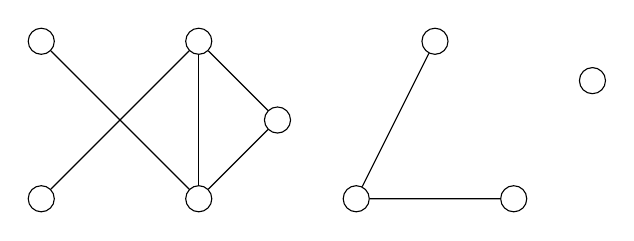
\begin{tikzpicture}
        \node [node] (1) at (0,2) {};
        \node [node] (2) at (2,2) {};
        \node [node] (3) at (0,0) {};
        \node [node] (4) at (2,0) {};
        \node [node] (5) at (3,1) {};

        \node [node] (6) at (5,2) {};
        \node [node] (7) at (4,0) {};
        \node [node] (8) at (6,0) {};

        \node [node] (9) at (7,1.5) {};

        \draw (1) -- (4) -- (5) -- (2) -- (3);
        \draw (2) -- (4);

        \draw (6) -- (7) -- (8);
    \end{tikzpicture}
\end{center}
In this course, we make the following assumptions:
\begin{itemize}
    \item The number of vertices is finite.
    \item No `multiple edges': every pair of vertices is connected by at most one edge.
    \item No loops: no vertex can be joined to itself - edges have to go between different vertices.
\end{itemize}

\subsection{Where do such structures arise?}
(Insert Konigsberg picture here)

\begin{eg}
    \leavevmode
    \begin{enumerate}[label=\arabic*.]
        \item Problem: Can we walk across each bridge in this city precisely once, returning to our starting point? (Euler, 1736)

            We turn the problem into a graph problem - in particular, a multigraph to allow multiple edges between vertices.  The vertices of this graph are the four bits of the city, while the edges are the seven bridges.
            In terms of this graph, the problem becomes to walk around the edges of this graph precisely once, and return to the starting vertex.

        \item Map colouring problem (1850s)

            How many colours are required to colour a map such that neighbouring countries get different colours?
            (picture)
            Here, the vertices are countries, and the edges are neighbouring pairs.  If we can draw a graph with no crossing edges, how many colours are needed to colour vertices with all edges having two different colours?

        \item Cosets of finite subgroups of finite groups

            Let $G$ be a finite group, $H \leq G$, $|G : H| = n$.  By Lagrange, $\exists a_1, \dots, a_n \in G$ such that the left cosets of $H$ are $a_1 H, \dots a_n H$.
            Similarly, $\exists b_1, \dots, b_n \in G$ such that the right cosets of $H$ are $H a_1, \dots, H a_n$.
            Can we do this simultaneously? In particular, are there $a_1, \dots, a_n \in G$ such that $a_1 H, \dots, a_n H \in G$ are the left cosets, and $H a_1, \dots, H a_n \in G$ are the right cosets?

            In the case where $H \lhd G$ this is easy since we have $a H = H a \; \forall a \in G$.  However it is less obvious if $H \centernot\lhd G$.
            Let $L$ be the set of left cosets, and let $R$ be the set of right cosets. We can create a graph where the vertices are $L \cup R$.
            Join $X \in L$ to $Y \in R$ by an edge if we can find some $a$ such that $X = aH$ and $Y = Ha$, that is, if $X$ and $Y$ have a common element.  Ideally, we would like a graph like this
            (insert bipartite graph here)

            Formally, we ask: In this graph, can we find a set of edges meeting each vertex precisely once?

        \item Fermat equation mod p

            Consider the equation $x^n + y^n = z^n$. Does this have solutions mod $p$ for $p$ a prime?  Rule out trivial solutions such as $x = 0, y = z$, in particular we search for solutions in $\mathbb{Z}_p$ where $xyz \ne 0$.
            Let $G = \mathbb{Z} \setminus \{0\}$ under multiplication, and $H = \{g^n : g \in G\}$.  We can check that $H \leq G$, and that $|G : H| \leq n$, by considering the number of $n$th roots an element can have.
            So, $G$ can be partitioned into $g_1 H, g_2 H, \dots, g_mH$ for some $g_1, g_2, \dots, g_m$ and $m \leq n$.  Suppose in some $g_i H$, we have $a, b, c$ with $a + b = c$.  Then $a = g_i x^n, b = g_i y^n, c = g_i z^n$ for some $x, y, z \in G$.  Then
            \begin{align*}
              g_i x^n + g_i y^n = g_i z^n \\
              x^n + y^n = z^n
            \end{align*}

            It finally remains to show Schur's Theorem:

            \begin{thm}[Schur's Theorem\label{thm:schur}]
                Let $n$ be a positive integer. Then if $p$ is a sufficiently large positive integer, whenever $\{1, 2, \dots, p\}$ is parititioned into $n$ parts, we can solve $a + b = c$ with $a, b, c$ all in some part.
            \end{thm}
    \end{enumerate}
\end{eg}

\clearpage
\section{Ramsey Theory}

\begin{defi}[Graph\hypertarget{def:graph}]
    A \textbf{graph} is an ordered pair $(V, E) = G$ where $V$ is a finite set and $E$ is a set of unordered pairs of distinct elements of $V$.
    We call elements of $V$ \textbf{vertices} of $G$ and elements of $E$ \textbf{edges}.
    We often write $v \in G$ to mean $v \in V$ and sometimes, where clear, $e \in G$ to mean $e \in E$.  Often denote $\{u, v\} \in E$ by $uv$. Note $uv = vu$.
\end{defi}

\begin{eg}
    Here's an example of a \hyperlink{def:graph}{graph} $G = (\{1, 2, 3, 4, 5, 6, 7\}, \{12, 23, 13, 14, 67\})$, but it's often easier to represent a graph by a drawing: take a point for each vertex, join two vertices if they are in an edge.
    \begin{center}
        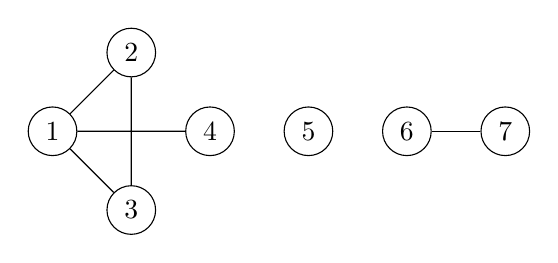
\begin{tikzpicture}
            \node [node] (1) at (-1, 0) {1};
            \node [node] (2) at (0, 1) {2};
            \node [node] (3) at (0, -1) {3};
            \node [node] (4) at (1, 0) {4};

            \node [node] (5) at (2.25, 0) {5};
            \node [node] (6) at (3.5, 0) {6};
            \node [node] (7) at (4.75, 0) {7};

            \draw (4) -- (1) -- (2) -- (3) -- (1);
            \draw (6) -- (7);
        \end{tikzpicture}
    \end{center}
\end{eg}

\begin{defi}[Graph isomorphism]\hypertarget{def:gIso}
    Let $G = (V, E)$ and $G' = (V', E')$ be \hyperref{def:graph}{graphs}. An \textbf{isomorphism} from $G$ to $G'$ is a bijection $\phi: V \to V'$ such that for all $u, v \in V$, we have $\phi(u) \phi(v) \in E'$ if and only if $u v \in E$.  If such an isomorphism exists, we say $G$ is isomorphic to $G'$.
\end{defi}

\begin{defi}[Subgraph]\hypertarget{def:subgraph}
    Suppose also $H = (W, F)$ is a graph. We say $H$ is a \textbf{subgraph} of $G$ and write $H \subset G$ if $W \subset V$ and $F \subset E$.  Often, we say `$H$ is a subgraph of $G$' to mean `$H$ is isomorphic to a subgraph of $G$'.
\end{defi}

\begin{defi}[Complete graph of order $n$]\hypertarget{def:Kn}
    The \textbf{complete graph of order n}, $K_n$ has $n$ vertices with every pair forming an edge.
\end{defi}

% add pictures of K1, K3, K5
\begin{center}
    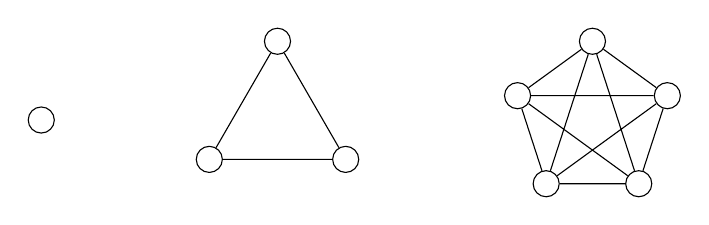
\begin{tikzpicture}
        \begin{scope}
            \node [node] (A) at (0, 0) {};
        \end{scope}

        \begin{scope}[xshift=3cm]
            \node [node] (A) at (  90:1)  {};
            \node [node] (B) at (-150:1)  {};
            \node [node] (C) at ( -30:1)  {};

            \draw (A) -- (B) -- (C) -- (A);
        \end{scope}

        \begin{scope}[xshift=7cm]
            \node [node] (A) at (  90:1)  {};
            \node [node] (B) at ( 162:1)  {};
            \node [node] (C) at (-126:1)  {};
            \node [node] (D) at ( -54:1)  {};
            \node [node] (E) at (  18:1)  {};

            \draw (A) -- (B) -- (C) -- (D) -- (E) -- (A);
            \draw (A) -- (C) -- (E) -- (B) -- (D) -- (A);
        \end{scope}
    \end{tikzpicture}
\end{center}

Looking at (fig), we see $K_3$ looks like a triangle, and we will often just refer to $K_3$ as a \textbf{triangle}\label{def:triangle}.  In addition, note that if $m \leq n$, then $K_m \subset K_n$.

Recall \nameref{thm:schur}:
\begin{thm}[Schur's Theorem reformulated]
    Let $k$ be a positive integer. Then there is a positive integer $n$ such that if the set $[n] = \{1, 2, \dots, n\}$ is coloured with $k$ colours, we can find $a, b, c$ with $a + b = c$ and $a,b,c$ the same colour.
\end{thm}

Can we prove this directly? First try $k=1$, where $n=2$ immediately works because $1+1=2$.

For $k=2$, (add stuff here). (blue 1, yellow 2, yellow 3, blue 4, any 5)
This case analysis worked for $k=2$, but is likely to get a lot more fiddly for larger $k$. Even for $k=3$ this case analysis turns out to be a lot harder, so can we come up with a `better' proof for the $k=2$ case, that is `more likely to generalise'?

\begin{proof}[$k=2$ of Schur's Theorem, improved]
    Suppose $[5]$ are coloured blue/yellow.  Then some three are the same colour, and without loss of generality $i < j < k$ are blue. If $j-i$ is blue we are done, since $i + (j-i) = j$.
    Similarly if $k-i$ or $k-j$ is blue, we are done.  If not, all of $j-i$, $k-i$, $k-j$ are all yellow, but then $k-i = (j-i) + (k-j)$, and we are done.
\end{proof}

Let's try a similar approach for $k=3$, and I claim $n=16$ works.

\begin{proof}(Schur's theorem, $k=3$)

    Suppose $[16]$ are coloured blue, yellow and green.  By the pigeonhole principle, some six numbers are the same colour, without loss of generality $x_1 < x_2 < \dots < x_6$ are blue.
    If $x_j - x_i$ is blue for any $i<j$ then we are done: $x_i + (x_j - x_i) = x_j$.  So assume all $x_j - x_i$ are green or yellow.
    Consider the five numbers $x_2 - x_1$, $x_3 - x_1$, $x_4 - x_1$, $x_5 - x_1$, $x_6 - x_1$.  By the $k=2$ case, some three of these are the same colour: say $x_i - x_1$, $x_j - x_1$, $x_k - x_1$ are yellow, for $i < j < k$.
    % (begin star)
    If $x_j - x_i$ is yellow, we are done: $(x_i - x_1) + (x_j - x_i) = x_j - x_1$, similarly if $x_k - x_i$ or $x_k - x_j$ is yellow.
    Otherwise, all of $x_j - x_i$, $x_k - x_i$, $x_k - x_j$ are all green, and we have $(x_j - x_i) + (x_k - x_j) = x_k - x_i$, so we are done.
    % (end star)
\end{proof}

This (star) looks very similar to the proof of the $k=2$ case, so can we use induction? It's unclear, because it wasn't exactly the previous case.  But notice how we always seem to be interested in differences of two numbers, yet we never seem to use facts like $7-3 = 9-5$.
So, consider a graph where the vertices are numbers, and the edges refer to the difference between two vertices, and we colour edges.
Suppose the edges of a complete graph $K_6$ are coloured blue and yellow. Then we can find a monochromatic \hyperref[def:triangle]{triangle}.
\begin{proof}
    Pick $v \in K_6$. $v$ is in five edges, so some three are the same colour, without loss of generality call them $vx, vy, vz$. If any of $xy, xz, yz$ is blue, we have a blue $triangle$ with $v$. If not, $xyz$ is a yellow triangle.
\end{proof}

\begin{remark}
    Schur for $k=2$ now follows: Suppose $[5]$ are coloured blue/yellow. Take a $K_6$ with vertices $\{0, 1, \dots, 5\}$. Colour edge $ij$, $(i<j)$ with the colour of $j-i$. By (ref), we have a monochromatic triangle $abc$ ($a<b<c$). Then $(c-b) + (b-a) = c-a$, and $c-b, b-a, c-a$ are all the same colour.
    We cannot find a monochromatic triangle in $K_5$ instead (picture)
    In this graph form, the statement for more colours is now amenable to an induction proof.
\end{remark}

% prop 1
\begin{nprop}
    Let $k$ be a positive integer. THen there is a postiive integer $n$ such that whenever the edges of $K_n$ are coloured with $k$ colours we can find a monochromatic triangle.
\end{nprop}

\begin{proof}
    Induction on $k$. For $k=1$, $n=3$ works.
    $k>1$. By the induction hypothesis, we can find $m$ such that if $K_m$ is $(k-1)$--coloured, then there is a monochromatic triangle.  Let $n = k(m-1) + 2$.

    Now $k$--colour the edges of $K_n$.  Pick vertex $v$.  The number of edges containing $v$ is $n-1 = k(m-1)+1$.  So some $m$ of them are the same colour, without loss of generality blue.  Let $H$ be a $K_m$ joined to $v$ by blue edges. If $H$ contains a blue edge, it makes a blue triangle with $v$. If not, $H$ is a $(k-1)$--coloured $K_m$ so by definition of $m$, it contains a monochromatic triangle.
\end{proof}

\begin{remark}
    \leavevmode
    \begin{enumerate}
        \item Can think in terms of the following picture. Eventually, we will run out of colours and get a monochromatic triangle.
        \item How big do we need to take $n$ to be?  Let $f(k)$ be the smallest $n$ that works with $k$ colours. Clearly $f(1) = 3$. Our proof says for $k>1$, $f(k) \leq k \left(f(k-1)-1\right) + 2 \leq k f(k-1)$.  So by induction, $f(k) < 3 k!$.
        \item Schur's theorem (add link) follows immediately in the same way as for the $k=2$ case.
    \end{enumerate}
\end{remark}

Can we find larger monochromatic subgraphs, for instance a monochromatic $K_4$?  Think about two colours at first for simplicity.  Yes, but need an intermediate step first.

\begin{eg}
    \leavevmode
    \begin{enumerate}
        \item Let $K_{10}$ have edges coloured blue/yellow.
            Then there is a blue triangle or a yellow $K_4$.
            \begin{proof}
                Take a vertex $v$. It's in $9$ edges so either $v$ is in $4$ blue edges, or in $6$ yellow edges.
                $v$ is in $4$ blue edges
                If any edge between $w, x, y, z$ is blue, we have a blue triangle.
                If not, there are all yellow and we have a yellow $K_4$.

                $v$ is in $6$ yellow edges We know $H$ contains a monochromatic triangle. If it is blue, we are done.  If it is yellow, then it makes a $K_4$ with $v$ as required.
            \end{proof}
        \item Let $K_{20}$ be coloured blue/yellow. Then $\exists$ a monochromatic $K_4$.
            \begin{proof}
                Pick a vertex $v$. It's in $19$ edges, so some $10$ of them are the same colour, without loss of generality blue.
                Let $H$ be a $K_{10}$ joined to $v$ by blue edges.
                Either $H$ has a blue triangle, making a blue $K_4$ with $v$
                Or $H$ contains a yellow $K_4$
            \end{proof}
    \end{enumerate}
\end{eg}

\begin{defi}[\hypertarget{def:ramseyNum}{Ramsey number}]
    Let $s, t \geq 2$. The Ramsey number $R(s, t)$ is the least $n$ such that whenever $K_n$ has edges coloured blue/yellow there must be a blue $K_s$ or a yellow $K_t$ (if such an $n$ exists).
    We also write $R(s) = R(s, s)$.
\end{defi}

We have seen $R(3) = 6$; $R(3, 4) \leq 10$; $R(4) \leq 20$.

\begin{nthm}[Ramsey's Theorem\label{thm:ramsey}]
    $R(s, t)$ exists for all $s, t \geq 2$.  Moreover, if $s, t \geq 2$ then $R(s, t) \leq R(s-1, t) + R(s, t-1)$.
\end{nthm}

\begin{proof}
    Induction on $s+t$.

    For $s=2$, we have $R(2, t) = t$, because reasons.  Similarly $R(s, 2) = s$.
    In the case $s, t > 2$, let $a = R(s-1, t)$ and $b = R(s, t-1)$ which exist by the induction hypothesis.  Let $n = a+b$. Suppose $K_n$ has edges coloured blue/yellow.
    Pick $v \in K_n$, which is in $a+b-1$ edges, so either $v$ is in $a$ blue edges, or it is in $b$ yellow edges.
    \begin{enumerate}
        \item If it is in $a$ blue edges, let $H$ be the $K_a$ joined to $v$ be blue edges.  Now $a = R(s-1, t)$, so either $H$ has a blue $K_{s-1}$, making a blue $K_s$ with $v$, or $H$ has a yellow $K_t$, so done.
        \item $v$ is in $b$ yellow edges, and we can make the same argument with colours reversed.
    \end{enumerate}
\end{proof}

% cor 3
\begin{ncor}
    For all $s, t \geq 2$, $R(s, t) \leq 2^{s+t}$, so $R(s) \leq 4^s$.
\end{ncor}

\begin{proof}
    Induction on $s + t$.  Base cases $s=2$, $R(2, t) = t \leq 2^{2+t}$ and similar for $t=2$.
    For $s, t \geq 2$
    \begin{align}
        R(s, t) &\leq R(s-1, t) + R(s, t-1) \\
                &\leq 2^{s-1+t} + 2^{s+1-t} \\
                &= 2^{s+t}
    \end{align}
\end{proof}

A more careful version of the same proof gives $R(s) = \mathcal{O} (\frac{4^s}{\sqrt{s}})$ (Erdos-Szekeres 1935)
A harder proof gives an improvement to $R(s) = \mathcal{O}(\frac{4^s}{s})$ (Thomason 1988)
An even harder proof gives $R(s) = \mathcal{O}(\frac{4^s}{s^k})$ for any $k$ (Conlon 2009)
Is $R(s) = \mathcal{O}((3.999999999)^s)$? Unknown.

\begin{nthm}[Multicolour Ramsey Theorem{thm:multiRamsey}]
    Let $k \geq 1$ and $s \geq 2$. Then there exists some $n$ such that whenever the edges of $K_n$ are coloured with $k$ colours, we can find a monochromatic $K_s$.
\end{nthm}

\begin{proof}
    Induction on $k$. For the base case $k=1$, we can take $n=s$.

    For $k>1$, by the induction hypothesis we can find $M$ such that if $K_m$ is $(k-1)$-coloured, then there is a monochromatic $K_s$. Let $n = R(s, m)$ and colour $K_n$ with $k$ colours, including blue but not yellow. Re-colour by turning all non-blue edges yellow. By definition, of $n$, we have either
    \begin{itemize}
        \item A blue $K_s$, so done
        \item A yellow $K_m$. Then in the original colouring, this $K_m$ was $(k-1)$-coloured, so by definitin of $m$, it contains a monochromatic $K_s$.
    \end{itemize}
\end{proof}

\begin{remark}
    \begin{enumerate} % 1.
        \item We write $R_k(s)$ for the smallest $n$ that works. In particular $R_1(s) = s$ and $R_2(s) = R(s)$.
            Proof of theorem 4 will give $R_k(s) \leq 4^{s^{k-1}}$.
        \item What do we really mean by colouring?
            We have informally talked about `yellow edges' etc. More formally, we have a colouring of the edges of $G = (V, E)$ with $k$ colours is a function $c: E:[k]$. We mostly refer to the colours as `blue', `yellow' and so on.
            We say $H = (W, F)$ is monochromatic if $c \mid_F$ is constant.
    \end{enumerate}
\end{remark}

With any number of colours, we can find arbitrarily large monochromatic subgraphs. What about infinite ones?

\begin{defi}[Infinite graph]\hypertarget{def:infGraph}
    An \textbf{infinite graph} is an ordered pair $G = (V, E)$ where $V$ is an infinite set and $E$ is a set of unordered pairs of elements of $V$. Note, in our terminology, an infinite graph is not a graph.
\end{defi}

\begin{defi}[(Possibly infinite) graph]\hypertarget{def:dumbDefi}
    A \textbf{(possibly infinite) graph} is a graph or an infinite graph.
\end{defi}

\begin{defi}[Infinite complete graph]\hypertarget{def:kInf}
    $K_\infty$ is the infinite graph with a countably infinite vertex set and every pair of vertices forming an edge.
\end{defi}

Where it makes sense to do so, we carry terminology over from graphs to infinite graphs.

Suppose edges of $K_\infty$ are coloured blue/yellow. What can we find? By Ramsey, we can find a monochromatic $K_s$ for every finite $s = 1, 2, 3, \dotsc$. Note this doesn't immediately give a monochromatic $K_\infty$:
In the diagram, we see that for any finite $s$ we have a blue $K_s$ but no blue $K_\infty$.  (However in this example, there is a yellow $K_\infty$)

\begin{nthm}[Infinite Ramsey Theorem]\label{thm:infRamsey}
    Let $k \geq 1$. Whenever the edges of $K_\infty$ are $k$-coloured, we have a monochromatic $K_\infty$ subgraph.
\end{nthm}

\begin{proof}
    Take $v_1 \in K_\infty$.  The vertex $v_1$ is in infinitely many edges, so infinitely many edges from $v_1$ are the same colour.
    Let $A_1$ be an infinite set of vertices of $K_\infty$ such that for all $u \in A_1$, $v_1 u$ has colour $c_1$.
    Now pick $v_2 \in A_1$. SImilarly, we can find an infinite $A_2 \subset A_1$ such taht all edges $v_2 u$ for ($u \in A_2$) have colour $c_2$.
    Keep going. We get infinite seuqences $v_1, v_2, v_3, \dotsc$ of vertices, $c_1, c_2, c_3, \dotsc$ of colours and $A_1 \supset A_2 \supset A_3 \supset \dots$ such that
    \begin{itemize}
        \item for $i \geq 2$, $v_i \in A_{i-1}$
        \item for $i \geq 1$, for all $u \in A_i$, $v_i u$ is an edge of colour $c_i$.
    \end{itemize}
    In particular, if $i < j$ then $v_i v_j$ has colour $c_i$. Now, infinitely many of the $c_i$ are the same.
    Say $i_1 < i_2 < i_3 < \dots$ such that $c_{i_1} = c_{i_2} = c_{i_3} = \dotsc$.
    Consider $v_{i_1}, v_{i_2}, v_{i_3}, \dotsc$. Any edge between two of these vertices hasc colour $c_{i_1}$. So we have a monochromatic $K_\infty$.
\end{proof}

\begin{remark}
    This is often called a `two-pass proof'. On the first pass, we found a sequence of colours, and on the second pass we found infinitely many colours the same.
\end{remark}
\end{document}
